% erdos634_v3C.tex (companion to Paper W, erdos634_v3W.tex) -- version 3.0 (2026-10-19).  Self-contained companion to the version 2.2 paper (erdos634_primes_and_N200.tex).
% Labels (Rule 0): \PL = PROVED-in-Lean (kernel-checked, standard axioms only, no sorry); \PH = PROVED-by-hand (written proof, audited, not formalized);
%   \CE = COMPUTED-exact (exact finite computation or exact verification of an explicit tiling, not a Lean proof); \CP = CLAIMED-by-Paliy (his public claim, not re-proved here);
%   \CJ = CONJECTURE.
% Figures: PDF files in figures/ (built by a separate figure kit).
\documentclass[11pt,reqno]{amsart}
\usepackage[T1]{fontenc}
\usepackage{amsmath,amssymb,amsthm}
\usepackage[margin=1.1in]{geometry}
\usepackage{array}
\usepackage{longtable}
\usepackage{booktabs}
\usepackage{graphicx}
\usepackage{tikz}
\usetikzlibrary{arrows.meta,positioning}
\usepackage{hyperref}
\hypersetup{colorlinks=true,linkcolor=blue,citecolor=blue,urlcolor=blue}

\theoremstyle{plain}
\newtheorem{theorem}{Theorem}[section]
\newtheorem{lemma}[theorem]{Lemma}
\newtheorem{corollary}[theorem]{Corollary}
\newtheorem{proposition}[theorem]{Proposition}
\newtheorem{conjecture}[theorem]{Conjecture}
\theoremstyle{definition}
\newtheorem{definition}[theorem]{Definition}
\newtheorem{remark}[theorem]{Remark}
\newtheorem{example}[theorem]{Example}

\newcommand{\R}{\mathbb{R}}
\newcommand{\Z}{\mathbb{Z}}
\newcommand{\Q}{\mathbb{Q}}
\newcommand{\N}{\mathbb{N}}
\newcommand{\lab}[1]{\textup{[\textsc{#1}]}}
\newcommand{\PL}{\lab{proved in Lean}}
\newcommand{\PH}{\lab{proved by hand}}
\newcommand{\CE}{\lab{computed, exact}}
\newcommand{\CP}{\lab{claimed by Paliy}}
\newcommand{\CJ}{\lab{conjecture}}
\newcommand{\why}[1]{\par\smallskip\noindent\emph{Why it matters.} #1\par}
\DeclareUrlCommand{\lean}{\urlstyle{tt}}
\newcommand{\tile}{\mathsf{tile}}
\newcommand{\kap}{\kappa}
\emergencystretch=2em

\title[Conjecture C, the collar family and the census]{Conjecture C, the collar family and the census of tile counts, with computer evidence\\ (companion to Paper~W)}
\author{Vico Bonfioli}
\date{Companion paper, version 3.0, 19 October 2026}

\begin{document}

%=====================================================================
\begin{abstract}
A positive integer $N$ is a \emph{tile count} if some triangle can be cut into $N$ pairwise congruent triangles (Problem 634 of \texttt{erdosproblems.com}). This is the companion of Paper~W \cite{PaperW}, which proves that the triangles $W_M(e,f)$ and $T_M(e,f)$ built from the tile $(ef,f^2-e^2,f^2)$ are tiled once $Me\ge f$ and $(M-1)(f-e)\ge f$ (Theorem~W); that theorem is used here, not proved.
This paper collects what surrounds it. (1) A \emph{collar family}: repeated one-layer steps give the tile counts $(f^2-1)(2f^2-1)g^2$ for $g\ge f+1$, and tails $465g^2$ ($g\ge5$ in Lean; $g=2,3,4$ by exact tilings), $966g^2$ and $2485g^2$ ($g\ge2$). (2) Twenty-six further tile counts by macro-piece layouts found by a template search, each with a Lean proof, and a twenty-seventh by square closure. (3) \emph{Conjecture C}, a candidate description of all tile counts as a union of explicit families: its existence half is proved on the ranges known, its exclusion half is open. (4) A census of the non-squarefree $N\le10^6$, by exact computation. (5) Computer evidence, not a proof, on one open family. (6) The \emph{thick regime}: Lean and hand no-tiling theorems for $W_M(e,f)$ when $M<f$, $Me\ge f$ and $M(f-e)\le e+2$, with the census effect, and a statement of what remains open. Every statement carries one of five labels (Lean, hand proof, exact computation, claimed by Paliy, conjecture); a list of corrections of earlier statements and a list of what is not proved are included. The prime case is not treated.
\end{abstract}
\maketitle

%=====================================================================
\section{Introduction}\label{sec:intro}

\subsection{The problem and what this paper adds}
A triangle $\Omega$ (the \emph{target}) is \emph{tiled by $N$ copies of a triangle $\tile$} (the \emph{tile}) if $\Omega$ is the union of $N$ closed triangles with pairwise disjoint interiors, each congruent to $\tile$; mirror images are allowed and the pieces need not meet edge to edge.
$N$ is a \emph{tile count} if some triangle is tiled by $N$ copies of some triangle (in the Lean statements, \texttt{TileCount N} says exactly this).
The squares, the numbers $x^2+y^2$, $3k^2$ and $6k^2$ are tile counts for classical reasons \cite{Soifer,SWW}.
Laczkovich classified the pairs (target, tile) up to the arithmetic of their angles \cite{Laczkovich1995,Laczkovich2012}; Beeson, with Ro\c{s}u, Zhang and Laczkovich, worked through the classes \cite{BeesonI,BeesonIII,BeesonIso,BeesonRosu,Zhang,Erdos633}.
Paliy published constructions and a proof of the prime case \cite{PaliyPrime,PaliyRepo}.
The earlier versions of this paper \cite{Release22,ReleasePaper} contain the exclusion side (the primes $p\equiv3\pmod4$, $p>3$, are not tile counts, a theorem of the earlier release that has been audited only inside the project, see Section~\ref{sec:notproved}; every $N\le200$ is decided; a census of the non-squarefree $N\le10^6$).
Version~3.0 is about the other side, \emph{which counts are tile counts}, and it is organised around one family of tiles, the one that carries every open question of the census.

\medskip\noindent\textbf{What we take from the earlier versions.} Four facts are used as black boxes, each a Lean theorem of the earlier release \cite{ReleasePaper,Release22} that is not reproved here: for the tile $\tile(e,f)$ of Section~\ref{sub:tile} and the target $W_M(e,f)$, $T_M(e,f)$ of Section~\ref{sub:targets},
(i) $W_M(e,f)$ is not tiled if $Me<f$ (called \texttt{cor:ebelow}(a)), and $T_M(e,f)$ is not tiled if $2Me<f$ (\texttt{cor:ebelow}(b));
(ii) $W_M(e,f)$ is not tiled if $M(f-e)\le e$ (\texttt{cor:thickw}(a));
(iii) for $e=1$ and for $e=f-1$ the scale $M=f$ is the threshold for $W_M$ (\texttt{cor:below}, \texttt{cor:thickw}(b));
(iv) $W_M$ and $T_M$ are tiled for every $M\ge f$ (Paliy, Beeson; formalized there).

\medskip\noindent\textbf{Standing of the statements.}
Every statement carries one of five labels:
\begin{itemize}\itemsep1pt
\item \PL{} a theorem of the accompanying Lean~4 library, checked by the kernel with the standard axioms only (\texttt{propext}, \texttt{Classical.choice}, \texttt{Quot.sound}), no \texttt{sorry}. The Lean statement has been compared with the mathematical one \emph{within this work only}; a reading by a person outside the project has not been made.
\item \PH{} a written proof, audited inside the project, not formalised.
\item \CE{} an exact finite computation, typically an explicit tiling whose pieces are listed in exact arithmetic and verified by an independent exact checker. For an explicit tiling this is a proof of existence, but not a Lean proof.
\item \CP{} a public claim of D.~Paliy that we have not re-proved (in some cases we have checked an example).
\item \CJ{} unproved.
\end{itemize}
Where a result has two labels (say, a hand proof and a Lean proof) both are given.

\subsection{Results at a glance}
In detail:
(1) \textbf{Theorem~W} (Paper~W \cite{PaperW}, Theorem 2.1; Lean and hand proof there): for $2\le e\le f-2$, $W_M(e,f)$ is tiled by $M^2(2f^2-e^2)$ tiles, and $T_M(e,f)$ by $M^2(3f^2-e^2)$ tiles, as soon as $Me\ge f$ and $(M-1)(f-e)\ge f$; stated here in Section~\ref{sec:thmW} and used, not proved.
(2) \emph{Collar family} (Lean): a collar construction for the isosceles target with base angles $\alpha$ gives, by repeated one-layer steps, the counts $(f^2-1)(2f^2-1)g^2$ for all $g\ge f+1$ ($f\ge2$), the tails $465\,g^2$ ($g\ge5$), $966\,g^2$ ($g\ge17$) and $2485\,g^2$ ($g\ge5$); together with the counts of (3) at small $g$ this gives $966g^2$ and $2485g^2$ for all $g\ge2$ (Lean). New: $465g^2$ for $g=2,3,4$ ($1860$, $4185$, $7440$) are tile counts of the tile $(4,15,16)$ by exact-verified tilings (not yet Lean), so $465g^2$ is a tile count for every $g\ge2$; the core $465$ ($g=1$) stays open. The up-set in $g$ was announced earlier by Paliy.
(3) \emph{Macro pieces}: twenty-six tile counts have individual Lean proofs, by macro-piece layouts found by a template search and verified exactly, and a twenty-seventh ($78\,246$) follows by square closure; twenty of them are values of $966g^2$ and $2485g^2$ at small $g$ (which complete the tails of (2); some also follow from others by Proposition~\ref{prop:square}), and seven are not ($375$, $540$, $735$, $825$, $630$, $1120$, $1750$). One hundred tilings are shipped as exact data.
(4) \textbf{Conjecture~C} (conjecture) states the set of tile counts as a union of explicit families; its existence half is a Lean theorem for the ranges proved so far (a collection narrower than the full table of families), and its exclusion half is open.
(5) \emph{Census} (exact computation, partly formal): for the non-squarefree $N\le10^6$, $199\,364$ values are excluded by Lean theorems (the assignment is made by a program; the theorems have been audited only inside the project), $129\,108$ are tile counts, $63\,602$ are undecided; counting the hand-proved Theorem~R2 class as well, $199\,441$ / $129\,108$ / $63\,525$; about $770$ squarefree values stay open. The three values $1860$, $4185$, $7440$ above were found after the census was run and are not in these numbers.
(6) \textbf{The thick regime} (Section~\ref{sec:thick}): for coprime $2\le e<f$, $M<f$, $Me\ge f$: $W_M(e,f)$ has no tiling if $M(f-e)\le e+1$ (Lean; hand proof audited inside the project; $124$ census values; formally in the exclusion chain: $412$, $270$), and, as a hand proof only, if $M(f-e)=e+2$ ($77$ more values).

The table gives the same results with their labels and places.
\begin{center}
\small
\begin{tabular}{@{}p{2.8cm}p{5.6cm}p{4.4cm}@{}}
\toprule
result & statement in one line & label and place\\
\midrule
Theorem W (Paper~W; \S\ref{sec:thmW} here) & $W_M(e,f)$ and $T_M(e,f)$ tile once $Me\ge f$ and $(M-1)(f-e)\ge f$ ($2\le e\le f-2$); Lean: the tiling for $W_M$, the count for $T_M$ & $W$ half \PL{} \PH{}; count of $T_M$ \PL{}; tiling of $T_M$ via an imported glue lemma; proved in Paper~W\\
Sharpness (Paper~W, Cor.~2.4) & for $2\le e<f/2$: $W_M(e,f)$ tiles iff $Me\ge f$ & ``if'' \PL{}; ``only if'' imported from the earlier release\\
Collar family (\S\ref{sec:collar}) & $(f^2-1)(2f^2-1)g^2$, $g\ge f+1$; tails $465g^2$ $(g\ge5$ \PL{}; $g=2,3,4$ \CE{} exact tilings only$)$, $966g^2$ and $2485g^2$ $(g\ge2$, using the macro counts at small $g)$ & \PL{}; collar step with arbitrary height \PH{}\\
Macro-piece counts (\S\ref{sec:macro}) & 27 further tile counts (e.g.\ $3864$, $9940$, $62125$, $279174$) & \PL{}, \CE{} data\\
Conjecture C (App.~\ref{sec:conjC}) & the set of tile counts is $\bigcup_k k^2\cdot\{\text{families}\}$ & existence half \PL{} on a narrower collection of proved ranges (App.~\ref{sec:conjC}); exclusion half \CJ{}\\
Census (App.~\ref{sec:census}) & $199\,364$ / $129\,108$ / $63\,602$ (non-squarefree $N\le10^6$; with the hand-proved class R2: $199\,441$ / $129\,108$ / $63\,525$) & \CE{} with label columns\\
Thick regime (\S\ref{sec:thick}) & $W_M(e,f)$ has no tiling for $e\ge2$, $M<f$, $Me\ge f$, $M(f-e)\le e+1$; and for $M(f-e)=e+2$ & first: \PL{} (hand proof audited inside the project); second: \PH{} only (arithmetic half in Lean)\\
$W^{3+}$ evidence (App.~\ref{app:w3}) & a set of candidate boundary words of a tiling of an isosceles target, defined in the appendix; for $(4,7)$, $(5,8)$ at $g=3$ no tiling was found for any of these words (a verdict conditional on hand-proved filters) & \CE{} (not formal)\\
\bottomrule
\end{tabular}
\end{center}

\begin{figure}[ht]
\centering
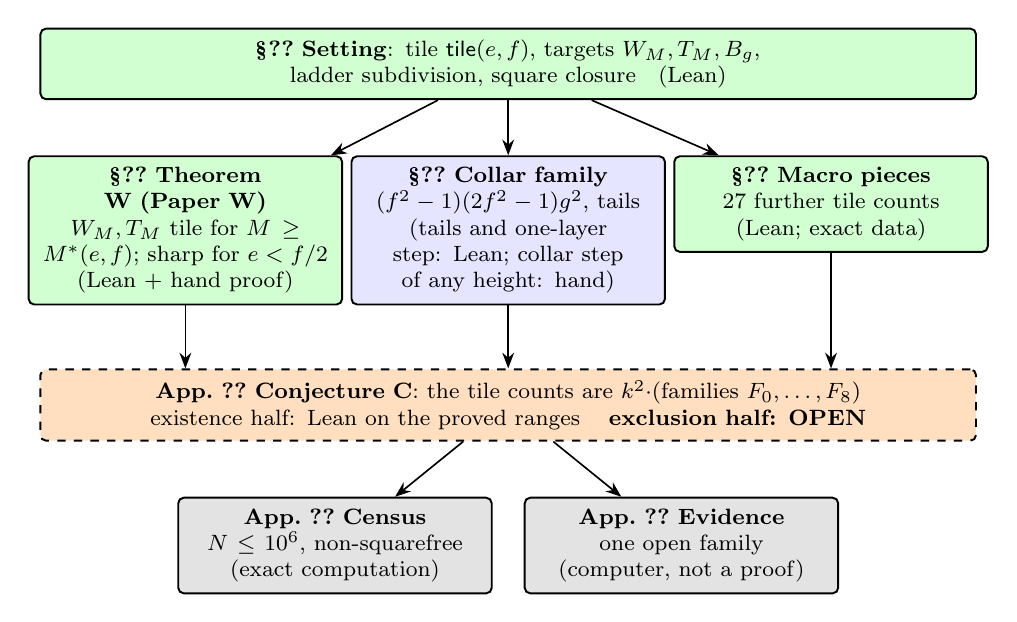
\begin{tikzpicture}[font=\footnotesize,node distance=5mm,
 box/.style={draw,rounded corners=2pt,align=center,inner sep=4pt,text width=3.7cm,line width=0.7pt},
 pl/.style={box,fill=green!18},ph/.style={box,fill=blue!10},ce/.style={box,fill=gray!22},cj/.style={box,fill=orange!25,dashed},
 arr/.style={-{Stealth[length=2mm]},line width=0.6pt}]
\node[pl,text width=11.6cm] (set) {\textbf{\S\ref{sec:setting} Setting}: tile $\tile(e,f)$, targets $W_M,T_M,B_g$, ladder subdivision, square closure \; (Lean)};
\node[pl,below=7mm of set,xshift=-4.1cm] (W) {\textbf{\S\ref{sec:thmW} Theorem W (Paper W)}\\ $W_M,T_M$ tile for $M\ge M^*(e,f)$; sharp for $e<f/2$\\ (Lean + hand proof)};
\node[ph,below=7mm of set] (C1) {\textbf{\S\ref{sec:collar} Collar family}\\ $(f^2-1)(2f^2-1)g^2$, tails\\ (tails and one-layer step: Lean; collar step of any height: hand)};
\node[pl,below=7mm of set,xshift=4.1cm] (Mac) {\textbf{\S\ref{sec:macro} Macro pieces}\\ 27 further tile counts\\ (Lean; exact data)};
\node[cj,below=8mm of C1,text width=11.6cm] (CC) {\textbf{App.~\ref{sec:conjC} Conjecture C}: the tile counts are $k^2\cdot$(families $F_0,\dots,F_8$)\\ existence half: Lean on the proved ranges \;\; \textbf{exclusion half: OPEN}};
\node[ce,below=7mm of CC,xshift=-2.2cm] (Cen) {\textbf{App.~\ref{sec:census} Census}\\ $N\le10^6$, non-squarefree\\ (exact computation)};
\node[ce,below=7mm of CC,xshift=2.2cm] (Ev) {\textbf{App.~\ref{app:w3} Evidence}\\ one open family\\ (computer, not a proof)};
\foreach \x in {W,C1,Mac} {\draw[arr] (set) -- (\x); \draw[arr] (\x) -- (CC.north -| \x);}
\draw[arr] (CC) -- (Cen); \draw[arr] (CC) -- (Ev);
\end{tikzpicture}
\caption{Map of the paper. Green: proved in Lean (Theorem~W has an additional hand proof); blue: hand proof (the collar step of arbitrary height; only height one and the tails are Lean); grey: exact or computer evidence only; orange dashed: conjecture. Nothing in this paper decides which counts are \emph{not} tile counts beyond the earlier releases.}\label{fig:roadmap}
\end{figure}

\subsection{Reading guide}
The body of the paper (Sections~\ref{sec:setting}--\ref{sec:credits}) contains the new constructions: Section~\ref{sec:setting} defines the tile, the targets and the two tools used throughout (ladder subdivision, square closure); Section~\ref{sec:thmW} restates Theorem~W of Paper~W and what it does to this paper; Sections~\ref{sec:collar} and~\ref{sec:macro} give the collar family and the macro-piece counts; Section~\ref{sec:notproved} lists what is not proved and Section~\ref{sec:credits} gives credits with dates.
The appendices hold the material that is needed for checking or for context: Appendix~\ref{app:W} says where the proof of Theorem~W is (in Paper~W); Appendix~\ref{sec:conjC} states Conjecture~C, a candidate description of all tile counts, and what is proved about it; Appendix~\ref{sec:census} is the census; Appendix~\ref{app:w3} is computer evidence on one open family; Appendix~\ref{app:corr} lists corrections of earlier statements; Appendices~\ref{app:data}--\ref{app:repro} give the data, an index of the Lean statements and the reproduction commands.
Three levels: ten minutes (this introduction and Figure~\ref{fig:roadmap}); an hour (Sections~\ref{sec:setting}--\ref{sec:thmW} and the part of Section~\ref{sec:collar} you care about); an afternoon (the body and Appendix~\ref{sec:conjC}). Everything else is supplementary and can be skipped.

\subsection{Credit and the use of an AI system}
The constructions in Sections~\ref{sec:thmW}--\ref{sec:macro} build on those of D.~Paliy (the $W/\beta$ framework, caps and collars, the $\alpha$-isosceles up-set, seeds), M.~Beeson and G.~Ro\c{s}u (the targets $W$, $T$ and the methods), B.~Herdt, M.~Laczkovich, Y.~X.~Zhang and J.~P.~Harries; Section~\ref{sec:credits} says exactly which statement is whose, with dates.
These results were obtained with the help of an AI system (Claude, Anthropic); the questions and the directions were the author's, and the proofs have been checked in Lean or by hand as labelled; the provenance table is in the repository README.

%=====================================================================
\section{Setting}\label{sec:setting}

\subsection{The tile}\label{sub:tile}
Throughout, $e<f$ are coprime positive integers and
\[
a=ef,\qquad b=f^2-e^2,\qquad c=f^2,\qquad \kappa=b+c=2f^2-e^2 .
\]
The \emph{tile} $\tile(e,f)$ is the triangle with sides $a,b,c$; $\alpha,\beta,\gamma$ are its angles opposite $a,b,c$.
Heron's formula gives $16\,\mathrm{Area}^2=e^2b^2(4f^2-e^2)$, and one checks $c^2=a^2+bc$ and
\[
3\alpha+2\beta=\pi,\qquad \gamma=2\alpha+\beta,\qquad \cos\alpha=\frac{\kappa}{2c}.
\]
(In the classification of the earlier paper these are the tiles of ``type~(T)'', the family on which its prime case rests; nothing below depends on that.) That $(a,b,c)$ is a triangle follows from $a+b-c=e(f-e)>0$.
The angle $\alpha/\pi$ is irrational; this is not used below.
(Figure~\ref{fig:tile}.) Small examples: $(e,f)=(1,2)$ gives the tile $(2,3,4)$; $(2,3)$ gives $(6,5,9)$; $(2,5)$ gives $(10,21,25)$; $(1,4)$ gives $(4,15,16)$.
\begin{figure}[ht]
\centering
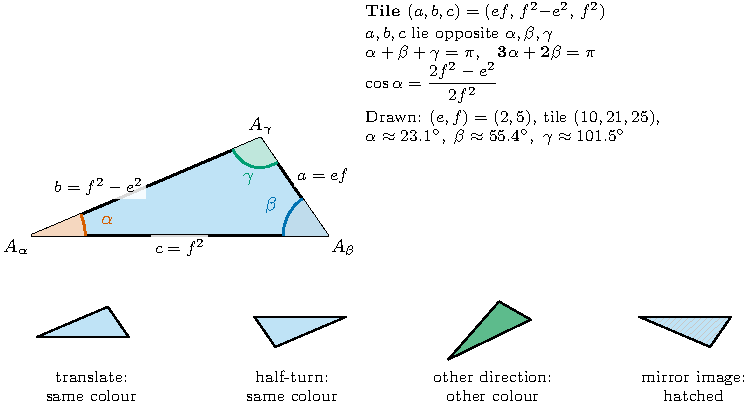
\includegraphics[width=0.85\linewidth]{figures/fig_tile.pdf}
\caption{The tile $\tile(e,f)$ with sides $a=ef$, $b=f^2-e^2$, $c=f^2$ and angles $\alpha$ (opposite $a$), $\beta$ (opposite $b$), $\gamma=2\alpha+\beta$ (opposite $c$), drawn for $(e,f)=(2,5)$, the tile $(10,21,25)$. The relation $3\alpha+2\beta=\pi$ is what makes the angles of the tile combine into the angles of the targets below. In all tiling figures that follow, tiles of the same orientation (up to a half-turn) share a colour, mirror images are hatched, and heavier lines are the boundaries between regions of one colour.}\label{fig:tile}
\end{figure}


\begin{table}[ht]
\caption{Symbols. This table is shared word for word with Paper~W \cite{PaperW}.}\label{tab:notation}
% notation_table.tex -- the ONE notation table shared by Paper W and the companion (version 3.0).  Edit here only.
% [W] = Paper W (Tilings of W_M and T_M below the threshold scale); [C] = the companion paper.
\begin{center}\small
\begin{tabular}{@{}p{2.6cm}p{9.9cm}@{}}
\toprule
symbol & meaning ([W] = Paper W; [C] = the companion paper)\\
\midrule
\multicolumn{2}{@{}l}{\emph{used in both papers}}\\
$e<f$ & coprime positive integers defining the tile; $d=f-e$\\
$a,b,c,\kappa$ & $a=ef$, $b=f^2-e^2$, $c=f^2$, $\kappa=b+c=2f^2-e^2$: the sides of the tile $\tile(e,f)$ and the sum $b+c$\\
$\alpha,\beta,\gamma$ & angles of the tile opposite $a,b,c$; $3\alpha+2\beta=\pi$, $\gamma=2\alpha+\beta$\\
scale $s$ & a triangle with sides $sa,sb,sc$ has \emph{scale} $s$ and is tiled by $s^2$ tiles (ladder subdivision, [W])\\
$W_M$, $T_M$ & the two targets of [W]; $M$ is the \emph{scale} of the target; $W_M$ is tiled by $M^2(2f^2-e^2)$ tiles, $T_M$ by $M^2(3f^2-e^2)$\\
$M^*(e,f)$ & threshold scale $\max(\lceil f/e\rceil,\lceil f/(f-e)\rceil+1)$ of Theorem~W; (H1), (H2) are $Me\ge f$ and $(M-1)(f-e)\ge f$, together equivalent to $M\ge M^*(e,f)$\\
\midrule
\multicolumn{2}{@{}l}{\emph{used in [W] only}}\\
$n,\rho,\delta$ & $n=\lfloor eM/f\rfloor$, $\rho=eM-fn$, $\delta=1$ if $\rho=0$ and $0$ otherwise\\
$t,r,q$ & the three free integers of the six-piece layout; canonical choice $t=n-\delta$, $r=n+1$, $q=n$\\
$\pi_0,\dots,\pi_5$ & the six pieces of the layout; $O,A,B,P,Q,R,\dots$ its points\\
\midrule
\multicolumn{2}{@{}l}{\emph{used in [C] only}}\\
$B_g$ & the isosceles target with base angles $\alpha$; $g$ is its scale; $b\kappa g^2$ tiles\\
row $(e,f)$ & the tile $\tile(e,f)$; $G(e,f)$ is the set of scales $g$ for which $B_g(e,f)$ is tiled\\
$F_0,\dots,F_8$ & the families of Conjecture~C\\
\bottomrule
\end{tabular}
\end{center}

\end{table}

\subsection{The targets}\label{sub:targets}
Let $M\ge1$ be an integer. The three families of targets that occur are listed in the table; the last column is the number of tiles that fit by area, which is the only count a tiling of the target can have.
\begin{center}
\small
\begin{tabular}{@{}llp{5.2cm}l@{}}
\toprule
target & sides & angles & area in tiles\\
\midrule
$T_M(e,f)$ & $Mf^3,\ Mf^3,\ Me(3f^2-e^2)$ & isosceles; apex $3\alpha$, base angles $\beta$ & $M^2(3f^2-e^2)$\\
$W_M(e,f)$ & $Mfb,\ Me\kappa,\ Mf^3$ & angles $2\alpha,\ \beta,\ \alpha+\beta$ (opposite $Me\kappa,\ Mfb,\ Mf^3$) & $M^2(2f^2-e^2)$\\
$B_g(e,f)$ & $gbc,\ gbc,\ gb\kappa$ & isosceles; base angles $\alpha$, apex $\alpha+2\beta$ & $b\kappa\,g^2$\\
\bottomrule
\end{tabular}
\end{center}
(For $W_M$, the side opposite the angle $2\alpha$ is $Me\kappa$, opposite $\beta$ is $Mfb$, and opposite $\alpha+\beta$ is $Mf^3$.)
$T_M$ and $W_M$ are the targets of Beeson--Ro\c{s}u and Paliy (``base-$\beta$'' targets); $B_g$ is the ``base-$\alpha$'' target (Paliy's $\alpha$-isosceles).
We call a target \emph{tiled} if it is tiled by copies of the tile $\tile(e,f)$ of the same $(e,f)$.
$W_M(e,f)$ and $T_M(e,f)$ are related by gluing: a tile at scale $Mf$ glued to the side $Mfb$ of $W_M$ gives $T_M$ (Paper~W, Proposition~2.3); all three are drawn in Figure~\ref{fig:targets}.
\begin{figure}[ht]
\centering
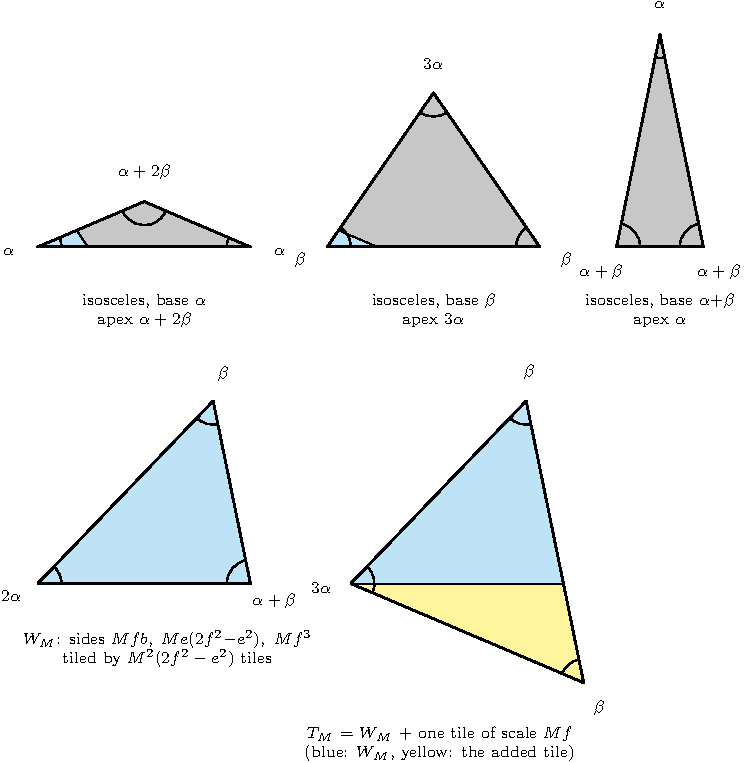
\includegraphics[width=0.8\linewidth]{figures/fig_targets.pdf}
\caption{The targets for $(e,f)=(2,5)$, $M=1$ proportions. Top: three isosceles shapes with base angles $\alpha$, $\beta$ and $\alpha{+}\beta$, with one tile placed at a base corner; the first is $B_g$, the second is $T_M$ in outline, and the third (base angles $\alpha{+}\beta$, apex $\alpha$) is the $\theta$-isosceles target of the family $F_8$ of Appendix~\ref{sec:conjC}, not used before that section. Bottom left: $W_M$ (angles $2\alpha$, $\alpha{+}\beta$, $\beta$), tiled by $M^2(2f^2-e^2)$ tiles. Bottom right: $T_M$, obtained from $W_M$ by adding one tile of scale $Mf$ along the side $Mfb$; it is the isosceles triangle with base angles $\beta$ and apex $3\alpha$, tiled by $M^2(3f^2-e^2)$ tiles. Angles are built from $\alpha,\beta$ by $3\alpha+2\beta=\pi$.}\label{fig:targets}
\end{figure}

\subsection{Two tools}\label{sub:tools}
\begin{proposition}[Ladder subdivision; \PL{}]\label{prop:ladder}
Let $s\ge1$ be an integer. A triangle similar to $\tile$ with sides $sa,sb,sc$ is tiled by $s^2$ copies of $\tile$.
A parallelogram with sides $sa$ and $uc$ enclosing the angle $\beta$ is tiled by $2su$ copies of $\tile$ (each unit cell is a parallelogram with sides $a,c$ enclosing $\beta$; the diagonal joining the far ends of those two sides has length $b$ and cuts the cell into two tiles).
\end{proposition}
\emph{Lean:} \lean{Subdivision.ladderDissection}, \lean{Ladder.ladder}; the earlier paper calls this \texttt{thm:ladder}.
A \emph{trapezoid} below means a triangle of scale $s_1$ minus a corner triangle of scale $s_2<s_1$ of the same shape (cut off by a line parallel to the opposite side); it contains $s_1^2-s_2^2$ tiles.
\begin{proposition}[Square closure; \PL{}]\label{prop:square}
If $N$ is a tile count then so is $k^2N$ for every integer $k\ge1$.
\end{proposition}
\emph{Lean:} \lean{TileCountFamilies.tileCount_scale}. (Enlarge the tiling of $\Omega$ by the factor $k$: this gives a tiling of a triangle $k\Omega$ by $N$ copies of the tile $k\tile$, with all sides multiplied by $k$. Each copy of $k\tile$ is a triangle of scale $k$ (sides $ka,kb,kc$), so by Proposition~\ref{prop:ladder} it is tiled by $k^2$ copies of the original tile $\tile$ itself. In total $k\Omega$ is tiled by $k^2N$ copies of $\tile$.)
\begin{remark}
In words: scaling the whole figure by $k$ multiplies the number of tiles by $k^2$.
Because of Proposition~\ref{prop:square} a tile count is naturally written $N=k^2n$, and thresholds below are thresholds in the \emph{scale of the target relative to the tile}, not in $k$.
\end{remark}


%=====================================================================
\section{Theorem W (of Paper W) and what it does here}\label{sec:thmW}
Everything in this section is proved in Paper~W \cite{PaperW}; the statements are restated so that the rest of this paper can be read alone. Notation: $M^*(e,f)=\max(\lceil f/e\rceil,\lceil f/(f-e)\rceil+1)$ and $d=f-e$.
\begin{theorem}[Theorem W; Paper~W, Theorem 2.1; $W$ half \PL{} and \PH{}, count of $T_M$ \PL{}, tiling of $T_M$ via a glue lemma of the earlier release]\label{thm:W}
Let $e,f$ be coprime with $2\le e\le f-2$ and $M\ge1$ with (H1) $Me\ge f$ and (H2) $(M-1)(f-e)\ge f$. Then $W_M(e,f)$ is tiled by $M^2(2f^2-e^2)$ copies of $\tile(e,f)$, and $T_M(e,f)$ by $M^2(3f^2-e^2)$ copies.
\end{theorem}
\begin{corollary}[Paper~W, Corollary 2.4; ``if'' \PL{}, ``only if'' imported from the earlier release]\label{cor:sharp}
For coprime $2\le e<f/2$, $W_M(e,f)$ is tiled if and only if $Me\ge f$.
\end{corollary}
\begin{corollary}[Paper~W, worked example in Section~5]\label{cor:W435}
$W_4(3,5)$, with sides $320,492,500$, is tiled by $656$ copies of $(15,16,25)$. The earlier paper listed this case as open.
\end{corollary}
\emph{Role here.} Theorem W supplies the family $F_1$ of Conjecture~C and $26\,138$ of the $26\,312$ new values of the census that are Lean theorems (Appendix~\ref{sec:census}; the rest of the $26\,312$ are the collar family, tails, macro counts, the thirteen witnesses and $k^2$-multiples); the proof (a layout of six pieces, with a table of every sign condition and the exact statement of what is Lean, hand, computed or imported) is Paper~W. The corrections that Paper~W makes to earlier expectations are listed in Appendix~\ref{app:corr}. What stays open for $W_M,T_M$ (the ``no'' side for $e>f/2$, $e=1$ and $e=f-1$ for $T_M$, the $T$ half in general) is stated in Paper~W, Section~6, and summarised in Section~\ref{sec:notproved}. The glue that gives $T_M$ from $W_M$ (one tile of scale $Mf$ on the side $Mfb$) is Paper~W, Proposition~2.3 (Section~2.2).

%=====================================================================
\section{The collar family and the base-$\alpha$ rows}\label{sec:collar}

This section is about the third target of Section~\ref{sub:targets}, the isosceles triangle $B_g(e,f)$ with base angles $\alpha$, legs $gbc$, base $gb\kappa$, and $b\kappa g^2$ tiles.
Write $N_0(e,f)=b\kappa=(f^2-e^2)(2f^2-e^2)$, so that a tiling of $B_g(e,f)$ has $N_0(e,f)g^2$ tiles; \emph{the row $(e,f)$} is the set of $g$ for which $B_g(e,f)$ is tiled.
The first values: $N_0(1,2)=21$, $N_0(2,3)=70$, $N_0(1,4)=465$, $N_0(2,5)=966$, $N_0(1,6)=2485$.
The row is non-empty in every case examined, and it is closed under addition (Paliy, \CP{}; his construction), so it is, if his claim holds, a numerical semigroup; what is open is its smallest element and its gaps.

\subsection{A priority statement}
D.~Paliy stated on 29 September 2026 \cite{PaliyRepo} that, for each tile, the targets $B_K$ (which have $b\kappa K^2$ tiles) are tiled for every $K$ beyond an explicit threshold $K_0$, so that the tile counts $b\kappa K^2$ are realised (the ``$\alpha$ up-set''); the seeds $84$ and $189$ of the row $(1,2)$ are in Beeson's work (the tilings of $84$ and $189$ in his Figures 28 and 29; $189$ is due to Harries).
\textbf{The up-set and the counts are Paliy's.}
What is ours in this section is an explicit construction of the layers (the \emph{collar}), a parametric seed for the whole family $e=1$, the explicit thresholds that follow, and their Lean proofs; the construction is independent of his, and the thresholds of Theorem~\ref{thm:tails} for the rows $(1,4)$ and $(1,6)$ are lower than the ones obtained from his formula as we read it, and for $(2,5)$ our tail coincides with his before the macro counts of Section~\ref{sec:macro} fill the smaller $g$ (we have not asked him about these readings).

\subsection{The collar step}
\begin{theorem}[Collar step; \PH{}, with a \PL{} one-layer case]\label{thm:collar}
Let $e<f$ be coprime, $a=ef$, $b=f^2-e^2$, $\kappa=2f^2-e^2$, and suppose $B_{g_0}(e,f)$ is tiled. Choose $\sigma\in[0,a)$ with $b\sigma\equiv b\kappa g_0\pmod a$ (it exists since $\gcd(a,b)=1$), put $K=(b\kappa g_0-b\sigma)/a$ and $h_{\max}=\lfloor K/a\rfloor$.
Then for every integer $h$ with $1\le h\le h_{\max}$ the triangle $B_{g_0+h}(e,f)$ is tiled.
\end{theorem}
\emph{Construction.} $B_{g_0+h}$ is a homothetic copy of $B_{g_0}$ at the apex plus a trapezoidal strip along the base; the strip is cut into three pieces by two lines, each tiled by Proposition~\ref{prop:ladder}: a triangle of scale $ch$, the difference of two triangles $\Delta(K)\setminus\Delta(K-ah)$, and the difference $\Delta(\sigma+bh)\setminus\Delta(\sigma)$.
The identity that makes the cut edges coincide is $c^2h+a(K-ah)=b\kappa(g_0+h)-b(\sigma+bh)$, which reduces to $c^2-a^2=bc$; the range $h\le K/a$ is exactly the condition $K-ah\ge0$.
\emph{Status.} The hand proof was audited independently (verdict: sound; checked exactly on $17\,853$ instances, all coprime $e<f<40$ with several $(g_0,h)$ each, and no failure). \PL{} The case $h=1$, for every row with $ef\le f^2-e^2$, is Lean \lean{Draft.CollarFam.layer_step} (real-level core \lean{Draft.CollarLayer.layer_core}); arbitrary $h$ is hand.
The corollary ``$g_0$ in the row implies every $g\ge g_0$ is in the row'' needs $h_{\max}(g_0)\ge g_0-1$ together with $h_{\max}(x)\ge1$ for $x\ge2g_0-1$ (both conditions are needed; see Appendix~\ref{app:corr}); it holds for the rows below. Figure~\ref{fig:collar} shows a collar around a seed.

\begin{figure}[ht]
\centering
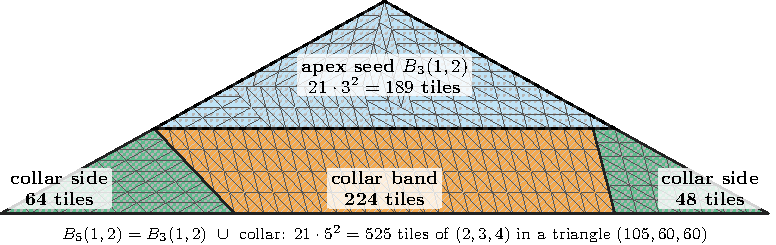
\includegraphics[width=1.0\linewidth]{figures/fig_collar.pdf}
\caption{The collar construction for the tile $(2,3,4)$ (row $(1,2)$): the triangle $B_5(1,2)$ with $525=21\cdot5^2$ tiles is an apex seed $B_3(1,2)$ ($189$ tiles, the top triangle) together with a collar of $336$ tiles (a band along the base and two side pieces). Colours are orientation classes. This is the picture of what the tiling contains; the step of Theorem~\ref{thm:collar} for general $g_0,h$ cuts the strip into three ladder pieces as described in the text.}\label{fig:collar}
\end{figure}

\subsection{The seed for $e=1$}
\begin{theorem}[Seed and up-set for $e=1$; \PL{}]\label{thm:seedA}
For every $f\ge2$ and every $g\ge f+1$, $\,(f^2-1)(2f^2-1)\,g^2$ is a tile count; the tiling is of $B_g(1,f)$ by copies of $(f,f^2-1,f^2)$.
\end{theorem}
\emph{Lean:} \lean{Draft.CollarUp.tileCount_e1_up}. The seed $g=f+1$ is a six-piece layout whose pieces are polynomial in $f$ (generated and checked symbolically; module \texttt{CollarSeed}, $125$ lemmas), and the layer step then gives all $g\ge f+1$.
For $f=2,3,4,6$ the seed counts are $189$, $2176$, $11\,625$, $121\,765$; the first is the $189$ of Beeson and Harries, the third and fourth were found by a template search in release v1.16.
\why{The sporadic-looking counts $189$, $11\,625$, $121\,765$ of earlier releases are the first members of one family, and the count $(f^2-1)(2f^2-1)g^2$ is a tile count for all $f\ge2$ at scales that no longer depend on a search.}

\subsection{Tails for three rows}
\begin{theorem}[Tails; \PL{}]\label{thm:tails}
(a) $465\,g^2$ is a tile count for every $g\ge5$ (row $(1,4)$, tile $(4,15,16)$).
(b) $2485\,g^2$ is a tile count for every $g\ge2$ (row $(1,6)$, tile $(6,35,36)$).
(c) $966\,g^2$ is a tile count for every $g\ge2$ (row $(2,5)$, tile $(10,21,25)$).
\end{theorem}
\emph{Lean:} (a) \lean{Draft.CollarFam.tileCount_465_sq}, from the seed $11\,625$ and the layer step. (b) The tail $g\ge5$ is \lean{Draft.CollarFam5.tileCount_2485_sq5}; $g=2,3$ are $9940$ and $22\,365$ (Section~\ref{sec:macro}), and $g=4$ is $4\cdot9940$ by Proposition~\ref{prop:square}. (c) The tail $g\ge17$ is \lean{Draft.CollarFam17.tileCount_966_sq17}; $g=2,\dots,8$ and $10,\dots,18$ are the macro-piece counts $3864,\dots,312\,984$ of Section~\ref{sec:macro} (sixteen values), and $g=9$ is $9\cdot8694=78\,246$ (\lean{Draft.AllMacro.tileCount_78246}).
The squarefree cores $465$, $966$ and $2485$ themselves ($g=1$) are not tile counts known to us; they are among the open squarefree values.
\begin{remark}
In our working notes we had recorded the pattern ``the smallest scale of a row is $f+1$ for even $f$''. (b) refutes it (the row $(1,6)$, with $f=6$ even, contains $g=2$, as does the row $(1,2)$), and (c) shows that the row $(2,5)$ contains $g=2$ as well.
For $(1,4)$ the values $g=2,3,4$ ($1860$, $4185$, $7440$) are tile counts by exact-verified tilings of the base-$\alpha$ isosceles targets $B_g(1,4)$ (sides $240g,240g,465g$) by the tile $(4,15,16)$, found after the Lean work of this release (data files \texttt{tiling\_1860\_s3\_14\_run\_4\_15\_16\_g2} and the two others; the exact verifier says VERIFIED; \CE{}, not yet Lean; the Lean certificates and the use of $g_0=2$ as a seed of the layer step are planned). Hence $465g^2$ is a tile count for every $g\ge2$ ($g\ge5$ in Lean, $g=2,3,4$ exact only). The core $465$ ($g=1$) is open; an exact search of bounded depth found no closure.
The up-set in $g$ and the threshold $K_0\ge\lceil B/v\rceil$ are Paliy's; they are the reason $g\ge5$ is a Lean theorem for $(1,4)$, and the new exact seeds lower the threshold in practice. Paliy's threshold, read from his formula, is $K_0=17$ for $(2,5)$ (equal to our tail in (c) before the macro pieces fill $g=2,\dots,16$), $6$ for $(1,4)$ and $8$ for $(1,6)$ (we did not check these values with him).
\end{remark}

%=====================================================================
\section{Macro-piece tile counts}\label{sec:macro}

\subsection{The idea}
In the six-piece layout of Paper~W every piece is tiled by the ladder subdivision, that is, by a tiling of a \emph{triangle similar to the tile}.
A \emph{macro piece} is a piece that is a triangle similar, with integer ratio $k$, to the \emph{target} of a tiling already known: such a piece is tiled by $k^2n$ tiles if the known tiling has $n$ tiles (Lean: \lean{Draft.MacroPiece.macroTFam_gen}, which transports a known dissection by the ladder theorem and congruence of triangles with equal sides).
Macro pieces were used for a long time by hand (Laczkovich's macro-dissections, Herdt's $1125$; Section~6 of the version-2.2 paper), and they enlarge the set of layouts for which the area equation has integer solutions.
The layouts are found by a computer search over the combinatorial type of the layout and the integer scales of its pieces, with the equations solved exactly; a layout is then expanded to the full list of tiles, verified by an exact checker, and finally turned into a Lean module, whose proof is the same area-and-containment argument as in Theorem~W with the numbers of that layout.
Figure~\ref{fig:macro} shows one such composition. The search itself is not part of this release; what is shipped are the results: the exact tilings (ninety-seven files, Appendix~\ref{app:data}) and the Lean theorems.

\subsection{The counts}
\begin{theorem}[Macro-piece tile counts; \PL{}, \CE{} data]\label{thm:macro}
Each of the following is a tile count, as the statement \texttt{TileCount $N$} of a Lean theorem:
\begin{center}\small
\begin{tabular}{@{}p{4.3cm}p{2.5cm}p{2.5cm}p{3.1cm}@{}}
\toprule
values $N$ & form & tile & what is tiled\\
\midrule
$375$, $540$, $735$ & $15m^2$, $m=5,6,7$ & $(3,5,7)$ & equilateral triangles of side $75,90,105$\\
$825$ & $33\cdot5^2$ & $(3,5,7)$ & isosceles, sides $105,105,165$\\
$630$, $1120$, $1750$ & $70\,g^2$, $g=3,4,5$ & $(6,5,9)$, row $(2,3)$ & $B_g(2,3)$\\
$3864$, $8694$, $15\,456$, $24\,150$, $34\,776$, $47\,334$, $61\,824$ & $966\,g^2$, $g=2,\dots,8$ & $(10,21,25)$, row $(2,5)$ & $B_g(2,5)$\\
$96\,600$, $116\,886$, $139\,104$, $163\,254$, $189\,336$, $217\,350$, $247\,296$, $279\,174$, $312\,984$ & $966\,g^2$, $g=10,\dots,18$ & $(10,21,25)$ & $B_g(2,5)$\\
$9940$, $22\,365$, $62\,125$ & $2485\,g^2$, $g=2,3,5$ & $(6,35,36)$, row $(1,6)$ & $B_g(1,6)$\\
\bottomrule
\end{tabular}
\end{center}
That is $26$ values, and a twenty-seventh, $78\,246=9\cdot8694$, by Proposition~\ref{prop:square}.
\end{theorem}
\emph{Lean:} one module \texttt{Draft/TM$N$} (or \texttt{Draft/T62125}) per value, with \texttt{theorem tileCount\_$N$ : TileCount $N$}; aggregate \lean{Draft.AllMacro}. Each module fixes the layout, proves the shapes and the containment by the area-and-sign method, and does not use a tile list; the standard axioms only.
The exact tilings of all of them are in \lean{data/witnesses/v3_exact} (for $N=375$, \texttt{tiling\_375\_macro\_5\_3\_7\_g1}); they have been verified by an exact checker independently of the Lean proofs.
\why{Together with Theorem~\ref{thm:tails} these counts show that in two rows, $(2,5)$ and $(1,6)$, \emph{every} scale $g\ge2$ is realised; the squarefree cores of those rows are the only open members. The $15m^2$ values for $m=5,6,7$ are the seeds that Paliy used (\CP{}) for his claim that $15m^2$ is a tile count for every $m\ge4$.}
For the equilateral counts $15m^2$: $m=4$ ($240$) was already a Lean theorem, and so was every $m$ in the semigroup generated by $4$ and $9$ (earlier release).
The Lean theorem \lean{Draft.EqSemigroup.eqD_step} says that equilateral tilings of sides $15m_1$ and $15m_2$ by copies of $(3,5,7)$ give one of side $15(m_1+m_2)$; the seeds $4,5,6,7$ would therefore give every $m\ge4$ (this is Paliy's claim, \CP{}).
The new Lean theorems for $m=5,6,7$ state only \texttt{TileCount} and are not yet instances of the equilateral predicate used by \texttt{eqD\_step}, so ``$15m^2$ for all $m\ge4$'' is \emph{not} a Lean theorem here; the exact tilings (sides $75,90,105$) are verified, and $15m^2$ for the individual $m=5,6,7$ is Lean.

\begin{figure}[ht]
\centering
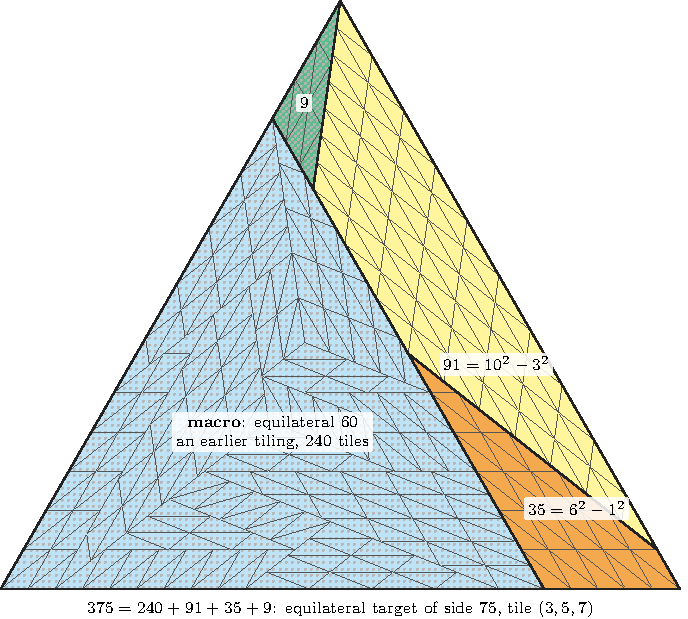
\includegraphics[width=0.75\linewidth]{figures/fig_macro.pdf}
\caption{Composition by macro pieces, for the equilateral triangle of side $75$ tiled by $375$ copies of $(3,5,7)$: the earlier $240$-tile tiling of the equilateral triangle of side $60$ (the seed, due to Paliy) is used as one block, and three further pieces of $91$, $35$ and $9$ tiles complete the triangle ($375=240+91+35+9$). The same method, with the macro piece a scaled copy of the target of a known tiling, produces the counts of Theorem~\ref{thm:macro} (here the ratio of the macro piece to its known target is $k=1$).}\label{fig:macro}
\end{figure}

\subsection{Other counts shipped in this release}
Twelve counts that are squares times earlier template counts ($46\,500$, $104\,625$, $267\,840$, $290\,625$, $418\,500$, $476\,160$, $487\,060$, $569\,625$, $602\,640$, $671\,460$, $744\,000$, $941\,625$; module \texttt{Draft/TemplateSquares}) are Lean theorems by Proposition~\ref{prop:square}; they were already tile counts mathematically and had been omitted by the census bookkeeping.
The thirteen tilings of $W_M$ with $M<f$ of Appendix~\ref{app:data} are also Lean theorems (\texttt{Draft/AllWBelow}), as are their upward closures (\texttt{Draft/AllDebtB}); they are subsumed by Theorem~W but were proved first.
$4830$ is a tile count: Paliy's certificate (4830 copies of $(24,11,31)$ tile the triangle $(961,1155,1426)$) has been converted and verified exactly (\CE{}; the construction is Paliy's, \CP{}; his family of mixed-corner layouts gives further values that we have not verified).


%=====================================================================
\section{What is not proved}\label{sec:notproved}
\begin{itemize}
\item \textbf{The exclusion half of Conjecture~C.} No description of the set of tile counts above $200$ is proved; the census has $63\,602$ undecided non-squarefree values ($63\,525$ if the hand-proved Theorem~R2 is accepted) and about $770$ squarefree values $\le10^6$.
\item \textbf{The no side of Theorem~W for $e>f/2$:} for each row exactly the scales $M$ with $(M-1)(f-e)<f<(M+1)(f-e)$ (at most two) are undecided; and \textbf{$e=1$ and $e=f-1$ for $T_M$} (for example $T_3(1,4)$); the $T$ side in general (only $2Me<f$ is excluded).
\item \textbf{$V$ and $A'$ for $\gamma=2\alpha$:} the evidence of Appendix~\ref{app:w3} is not a proof; $(7,12)$ is incomplete ($95.06\%$).
\item \textbf{$\Theta$ and $S_3$:} the thresholds of the $\theta$-isosceles family and of the base-$\alpha$ rows; the squarefree cores $465$, $966$, $2485$ ($g=1$); Lean certificates for the tile counts $1860$, $4185$, $7440$ (exact-verified only here).
\item \textbf{$15m^2$ for every $m\ge4$ as a Lean theorem}; the collar step for arbitrary height $h$ (hand only); Paliy's claims that we have not verified ($134$ values $\le10^6$ in the census; the mixed-corner family beyond $4830$).
\item \textbf{The squarefree values:} about $770$ open; the squarefree tile counts known to us are of the classical forms, or come from a short list of sporadic and layout values (the $22$ of the earlier release, $77$, $143$, $4830$).
\item \textbf{Outside check.} The Lean statements and the proofs have been compared and audited only inside this project, including the statement of \texttt{theoremP\_6} (the prime case of the earlier releases) and of Theorem~W; a check by a reader outside the project has not been made, and announcing the prime case as proved remains the author's decision.
\item \textbf{The thick regime beyond rung $e+2$:} for $M<f$, $Me\ge f$ and $M(f-e)\ge e+3$ (and $<f$) the question is open; Theorem~R2 is a hand proof read only inside the project; see Section~\ref{sec:thick}.
\item The search that found the macro layouts is not part of this release and is not described further than in Section~\ref{sec:macro}; its outputs are verified independently.
\end{itemize}


%=====================================================================
\section{The thick regime: no-tiling rungs}\label{sec:thick}
This section is about the scales $M$ below $f$ for which Theorem~W does not apply and the exclusion of the earlier release does not either. Write $d=f-e$ and let $2\le e<f$ be coprime. Theorem~W covers $M\ge M^*$; the earlier exclusion (I2 of Paper~W) covers $Md\le e$ and $Me<f$. The new statements push the exclusion to $Md\le e+2$, when $M<f$ and $Me\ge f$.
\begin{theorem}[rung $e+1$; \PL{} for the statement, hand proof audited inside the project]\label{thm:thick1}
Let $\gcd(e,f)=1$, $2\le e<f$, $M<f$, $Me\ge f$ and $M(f-e)\le e+1$. Then $W_M(e,f)$ is not tiled by copies of $\tile(e,f)$.
\end{theorem}
\emph{Lean:} \lean{Draft.SplusThick.wTilable\_not\_of\_small\_M} (module \texttt{SplusThickFinal}; aggregate \texttt{Erdos634.AllSplusThick}; standard axioms, no \texttt{sorry}). The proof studies the side $AQ$ of $W_M$ that ends at the corner $2\alpha$: the thick corner-run theorem (Lean \lean{Draft.SplusThick.cornerrun\_counts\_thick}) gives a representation of its length by $a,b,c$ with $z\ge e+1$ tiles having their $c$-edge on the side, and $z\ge e+2$ when $e+2\le f$, while the arithmetic of the side (Lean \lean{Draft.SplusThick.C\_AQ'}) gives $z\le M(f-e)\le e+1$; these contradict. The hand proof was audited inside the project (verdict: sound, with fixes now applied: the hypothesis $M<f$, and the arithmetic of $AQ$ for $M(f-e)<f$); nobody outside the project has read it.
\emph{Census.} There are $124$ non-squarefree values $N=M^2(2f^2-e^2)\le10^6$ that are excluded by this theorem and by no earlier one. They are census-level exclusions, except $N=412=W_2(5,8)$, which is a Lean theorem about $412$ itself: \lean{Draft.NSQM.no\_dissection\_412} (the S+ kill composed into the exclusion chain; modules \texttt{NSQRWT2}, \texttt{NSQMMainZETW2}, \texttt{NSQMMainZETWD2}). The value $270$ is a separate Lean exclusion (\lean{Draft.NSQM.no\_dissection\_270}, through the gap lemma for $30s^2$). The statement $W_2(5,8)$ was before this release the example of an open case with $e>f/2$ (Paper~W, Section~6): it is now excluded, so the ``computed, not proved'' search there is superseded.

\begin{theorem}[Theorem R2, rung $e+2$; \PH{} only]\label{thm:R2}
Let $\gcd(e,f)=1$, $2\le e$, $e+3\le f$, $M<f$, $Me\ge f$ and $M(f-e)\le e+2$. Then $W_M(e,f)$ is not tiled.
\end{theorem}
\emph{Status.} Hand proof, written out in \texttt{docs/THEOREM\_R2\_PROOF.md}. It was audited twice inside the project by readers of the same model family as the author (verdicts: sound with statement-level fixes, applied), re-checked by exact rational computation at twelve pairs $(e,f)$, and tested once by an exact region search at $(e,f,M)=(4,7,2)$, which did not refute it. It has \emph{not} been read by a person outside the project. Lean: only the arithmetic half (\lean{Draft.SplusR2.r2\_arith}) and a corollary that is \emph{conditional} on the geometric core, a statement \texttt{R2Count} that is not proved in Lean (\lean{Draft.SplusR2.wTilable\_not\_of\_small\_M2\_of\_R2}). So Theorem~R2 is not a Lean theorem, and the numbers that use it are reported in a separate row of the census.
\emph{Sketch.} A tiling of $W_M$ has a run $C_1^{k}$ of tiles with their $c$-edges on the side $AQ$ at the corner $2\alpha$; the earlier work shows $k\ge e+1$ and the case $k=e+1$ (Theorem~\ref{thm:thick1}). For $k=e+2$ one looks at the tile $S_0$ in the free wedge at the second lattice point of the run. If it is the mirror image $N_0(0)$ of the first run tile in its $a$-edge, the chord along its $c$-edge forces (partition property, $e\ge2$) a $b$-edge on the next line, and the row above the run is $c^e$ or $a^f$; arithmetic shows $c-b$ and $a-b$ are not in the semigroup $\langle a,b,c\rangle$, so the end of a lattice edge must lie inside an edge of a tile, and two tiles then overlap in a wedge of angle $\beta$ at that point. If $S_0$ is the half-turn image of the first tile, the row at level $1$ is $c^{e+1}$ or $c\,a^f$, and the second is killed by a size-one instance of the corner lemmas. The remaining call has size $e+1$ at level $1$ and is killed by the same two ideas. Hypotheses: $e\ge2$ (the representation of $c$ is unique), $e+3\le f$ (multipliers stay $\le f-1$).
\emph{Census.} For coprime $e<f\le40$, $M\ge2$, $Me\ge f$, $M(f-e)=e+2$ there are $26$ triples (first: $(4,7,2)$, $N=328$, and $(7,10,3)$, $N=1359$); the census program counts $77$ more excluded values $\le10^6$ with Theorem~R2: $199\,441$ / $129\,108$ / $63\,525$. The first rung not covered is $M(f-e)=e+3$: for $(5,9,2)$ and $(6,11,2)$.

\begin{lemma}[scale two; \PH{}, audited once inside the project]\label{lem:W2}
Let $e>f/2$, $\gcd(e,f)=1$, $g=f-e$, and suppose $W_2(e,f)$ is tiled. Then the side $OB$ (from the corner $2\alpha$ to the corner $\beta$; length $2fb$) carries exactly $2g$ tiles with an $a$-edge and $2g$ with a $c$-edge, and none with a $b$-edge; the corner run $C_1^k$ has $e+1\le k\le 2g$.
\end{lemma}
The proof is a congruence argument on the representation $2fb=xa+yb+zc$ together with the corner-run theorem of the earlier release (no representation with $z\ge f$ since $2g<f$). With Theorems~\ref{thm:thick1} and~\ref{thm:R2}: $W_2(e,f)$ has no tiling whenever $2g\le e+2$; what remains is the window $e+3\le k\le 2(f-e)$, with the smallest cases $(e,f)=(5,9)$ ($k=8$), $(6,11)$ ($k=9,10$), $(7,12)$ ($k=10$). This is \emph{not} proved: it is the open residual of the scale-two case.

\subsection*{Boundary words of the known tilings (computed)}
For all $37$ tilings of $W_M(e,f)$ and $15$ of $T_M(e,f)$ among the exact witnesses (all of them layouts of the template of Theorem~W) the three sides read, with $n=\lfloor eM/f\rfloor$, $\rho=eM\bmod f$, $\delta=[\rho=0]$ and $t=n-\delta$:
$OA=c^{fM}$, $OB=c^{fM-er}a^{fr-eM}$, $AB=a^{fM-et}c^{ft}b^{eM-ft}$, with $r\in\{n+1,M,M+1\}$ (the three values occurring). That is the vertex table of Theorem~W read backwards; the observation that only these three $r$ occur is \CE{} on $52$ witnesses and is not proved. The $b$-run on $AB$ is the least residue of $eM$ modulo $f$, in every witness. Every interior chain of collinear same-side edges is monochromatic or a word $c^pa^q$ or $a^pc^q$ (in $15\,678$ interior chains), so no Sturmian or Beatty word occurs on lines.
\emph{A Beatty form of the threshold} (identity, \CE{}: checked exactly for all $296\,736$ coprime triples with $2\le e\le f-2$, $f\le80$, $1\le M\le3f$, no mismatch; not proved here): with $n=\lfloor eM/f\rfloor$, ``$Me\ge f$ and $(M-1)(f-e)\ge f$'' holds if and only if $n\ge1$ and there is an integer $q\le M-1$ with $e(n+1)/f<q<fn/e$. So the threshold of Theorem~W says that this interval has caught an integer; below the threshold, for example $(5,9,2)$, $(6,11,2)$, $(7,12,2)$, it contains none. This restates the threshold and is not a new obstruction.

\subsection*{Dead routes, with data (notes, not proofs)}
(i) A conjectured lower bound $r\ge 2f-e$ for the corner run (``$R^*$'') is refuted by the scale-four witnesses $W_4(4,7)$, $W_4(5,9)$, $W_4(6,11)$, $W_4(7,12)$ ($r=8,11,14,13$, against $2f-e=10,13,16,17$). (ii) A conjectured bound on interior runs (``$S_\infty$'') is refuted by $2\,430$ interior runs in the witnesses. (iii) Describing the second layer of boundary words by a zigzag automaton gives a finite automaton ($K=f+1$ states) of positive entropy, so it cannot single out the tilings. (iv) Counts of Eisenstein-integer solutions and the windows for $\gamma=2\alpha$ were measured and gave no exclusion. (v) Reading a $W_2$ as a scale-two problem reduces it to the window of Lemma~\ref{lem:W2} and no further.
\textbf{What is not proved:} the exclusion for $M(f-e)\ge e+3$ (and $<f$), the no side of Theorem~W for $e>f/2$ in general, $T_M$ below $M^*$, and everything about the prime case.

%=====================================================================
\section{Credits, with dates}\label{sec:credits}
``Ours'': statement and proof produced in this work. ``Formalized'': another author's statement and construction, our Lean proof. Dates are of first public record (repository commit dates, arXiv versions) unless marked.
\begin{center}
\small
\begin{tabular}{@{}p{4.4cm}p{1.8cm}p{6.4cm}@{}}
\toprule
result & status here & whose, and when\\
\midrule
Prime counts; the base-$\beta$ reduction & earlier releases & Paliy, first public proof 2026-09-29 \cite{PaliyPrime}; ours independent; exclusion of $e=1$ public 2026-09-12 (an earlier Zenodo release, numbered v3.2 at the time); Beeson's withdrawal note for arXiv:2607.19572 (v2, 2026-09-24) \cite{BeesonWithdrawn} credits the author, cited here as public record\\
Targets $W_M$, $T_M$; tilings for $M\ge f$ & formalized & Paliy ($W/\beta$ framework, caps, collars: 2026-10-03; all $M\ge f$ (his $v$): 2026-10-10); Beeson and Ro\c{s}u (the targets, the seed)\\
\textbf{Theorem~W}, six-piece template & ours & template found by our search; the setting and the earlier thresholds are Paliy's and Beeson's; the sharpness side ($Me<f$) is from the earlier releases\\
$\alpha$ up-set, form $b\kappa K^2$, scale additivity & Paliy's; Lean here & Paliy, 2026-09-29 \cite{PaliyRepo}; seeds $84$, $189$: Beeson (Figs.~28--29), $189$: Harries\\
Collar step, parametric seed $e=1$, tails & ours & independent of Paliy's construction; credit for the up-set and the threshold $K_0$ as above\\
$465g^2$, $g=2,3,4$ (exact tilings) & ours (data) & seeds below Paliy's threshold; exact-verified, Lean planned\\
Thick regime (no tiling for $M(f-e)\le e+1$, hand proof of $e+2$) & ours & uses the run framework of Beeson and Ro\c{s}u and Paliy's $W/\beta$ setting; the arithmetic of the corner side and the partition property are from earlier releases\\
Macro pieces & ours (layouts, Lean) & macro-dissections: Laczkovich; Herdt ($1125$); seeds $15m^2$: Paliy (2026-10-08)\\
$15m^2$ for all $m\ge4$, $4830$, mixed-corner family & Paliy's (\CP{}); $4830$ verified here & Paliy, 2026-10-08\\
$990$, $264$, $897$, $240$, $312$ & earlier releases & Paliy: $990$ on 2026-10-06, $264$ on 2026-10-07; the others as dated in the earlier releases\\
$\theta$-isosceles family, scale additivity & Paliy's (\CP{}) & Paliy, 2026-09-29\\
Run induction, Theorem~F and $D'$ & earlier releases & method: Beeson and Ro\c{s}u (preprint of 2026-10-16); $g=1$: Beeson 2012\\
$1125$-tiling & earlier releases & Herdt, as published by Beeson \cite{BeesonRosu}\\
$88$ & earlier releases & Harries\\
$2\pi/3$ families $F_3$, $15m^2,33m^2$ & formalized & Zhang (arXiv:2512.22696); seeds Paliy, Herdt\\
Rep-tiling and $F_0$ & --- & Snover, Waiveris and Williams\\
Classification of pairs (triangle, tile) & --- & Laczkovich\\
Conjecture~C, census, $W^{3+}$ evidence & ours & ---\\
\bottomrule
\end{tabular}
\end{center}
The statements ``Paliy claims'' in this paper are statements in his public repository \cite{PaliyRepo}; we have read his documents and checked some examples, and we say so where we did. Nothing here is a claim of priority over him for the results listed as his; the dates are given so that the order is visible.


%=====================================================================
\appendix
\section{Where the proof of Theorem~W is}\label{app:W}
The proof of Theorem~W (coordinates, the six pieces, the sign table, the choice of parameters, the exact accounting of what is Lean, hand and computed) is in Paper~W \cite{PaperW}, Section~4 (with the worked rows in Section~5) and the separate verification record; the algebra is re-run by \texttt{code/check\_thmW\_algebra.py}. It is not repeated here.

%=====================================================================
\section{Conjecture C: a candidate classification of the tile counts}\label{sec:conjC}

The earlier papers give the exclusion side and a growing list of tile counts, but no statement of what the set of tile counts \emph{is}.
This section states one, as a conjecture, and says exactly what part of it is proved.
\textbf{It is not claimed to be true.} It is an organising map: a new tile count is either in a family (no news), or extends a family's range, or is a counterexample to the conjecture.

\subsection{The statement}
Recall Proposition~\ref{prop:square}: every family below is understood closed under $n\mapsto k^2n$.
\begin{conjecture}[Conjecture C; \CJ{}]\label{conj:C}
A positive integer $N$ is a tile count if and only if $N=k^2n$ for some integer $k\ge1$ and some core $n$ in one of the families $F_0,\dots,F_8$ of Table~\ref{tab:families}, with the parameter ranges stated there.
\end{conjecture}
\begin{table}[ht]
\small
\renewcommand{\arraystretch}{1.15}
\begin{tabular}{@{}p{0.55cm}p{3.2cm}p{3.3cm}p{5.1cm}@{}}
\toprule
 & cores $n$ & tile, target & range proved \quad (label) / credit\\
\midrule
$F_0$ & $1$, $x^2+y^2$ ($x,y\ge1$), $3$, $6$ & similar tiles, rep-tiles & all \quad \PL{} / Snover--Waiveris--Williams, Laczkovich\\
$F_1$ & $2f^2-e^2$ and $3f^2-e^2$, at scale $M$: $M^2(2f^2-e^2)$, $M^2(3f^2-e^2)$ & $\tile(e,f)$; $W_M$, $T_M$ & $e=1$ or $e=f-1$: $M\ge f$. $2\le e\le f-2$: $M\ge M^*(e,f)$ (Thm~\ref{thm:W}). \quad \PL{} / Paliy, Beeson ($M\ge f$); ours ($M^*$)\\
$F_2$ & $(2q^2-p^2)(3q^2-p^2)$, $0<p<q$ & five-piece layouts & all \quad \PL{} / Paliy\\
$F_3$ & $(2a+b)(a+b)$, $3(a+b)(a+2b)$, $(a+2b)(2a+b)$ and Zhang's five forms $\times m^2$; $15m^2$, $33m^2$ & tiles with an angle $2\pi/3$, $c^2=a^2+ab+b^2$; $(3,5,7)$ & ranges as in the Lean predicates; $15m^2$: $m\in\langle4,9\rangle$, and $m=5,6,7$ individually \quad \PL{} / Paliy, Zhang, Herdt. $15m^2$ for all $m\ge4$: \CP{}\\
$F_4$ & $88$, $143$ (sporadic) & tile $(3,5,7)$ on the triangles $(21,55,56)$ ($88$) and $(39,49,55)$ ($143$) & \PL{} / Harries ($88$); ours ($143$)\\
$F_5$ & $(f^2-e^2)(2f^2-e^2)\,g^2$, $g\in G(e,f)$ & $\tile(e,f)$; $B_g(e,f)$ & $e=1$: $g\ge f+1$; $(1,4)$: $g\ge5$; $(1,6),(2,5)$: $g\ge2$; $(2,3)$: $g=3,4,5$ and more by Thm~\ref{thm:collar} \quad \PL{} / \PH{}; Paliy: eventual up-set in every row, \CP{}\\
$F_6$ & $b\,(v(D+\tau v))^2$, positive integers $D,\tau$ (four more integers are subject to two linear Diophantine conditions, (E1), (E2) of the version-2.2 paper); $1125$, $19\,600$, $130\,977$ & $\gamma=2\alpha$, tile $(u^2,v^2-u^2,uv)$ & Herdt's family and its uniform version \quad \PL{} / Herdt, Laczkovich\\
$F_7$ & $4830$ & $(24,11,31)$ & \CE{} / Paliy, \CP{} (mixed-corner family)\\
$F_8$ & $b\,t^2$, $t\in S(e,f)$ & $\tile(e,f)$; $\theta$-isosceles target (legs $tfb$, base $teb$, base angles $\alpha+\beta$, $bt^2$ tiles) & \CP{} / Paliy (semigroup $S(e,f)$, $te\ge2f$ necessary \PL{})\\
\bottomrule
\end{tabular}
\caption{The families of Conjecture~C and what is proved about each. $\langle4,9\rangle$ is the set of non-negative combinations of $4$ and $9$. In $F_1$ the ranges are those of Theorem~\ref{thm:W} and of the earlier theorem for $M\ge f$; for the members $e=1$ and $e=f-1$ the threshold $f$ is proved sharp for $W_M$.}\label{tab:families}
\end{table}
\emph{Remarks.} (i) $84=21\cdot2^2$ and $189=21\cdot3^2$ are not sporadic: they are the members $g=2,3$ of the row $(1,2)$ of $F_5$ (earlier lists had them in $F_4$; $g=2$ is below the range $g\ge f+1=3$ proved in Theorem~\ref{thm:seedA}, so $84$ is an earlier-release value); $77\in F_2$; $183$ is \emph{not} a tile count (it is among the excluded values $\le200$; an earlier draft of this section listed it by a misreading, see Appendix~\ref{app:corr}).
(ii) Theorem~\ref{thm:W} is stated for $2\le e\le f-2$; $F_1$ in Table~\ref{tab:families} includes the two edge members with their threshold $f$.
(iii) For $F_6$ the earlier papers state two conjectures about its exclusion side, $V$ ($v\mid g$ is necessary) and $A'$ (a size bound); Appendix~\ref{app:w3} gives evidence for them.

\begin{figure}[ht]
\centering
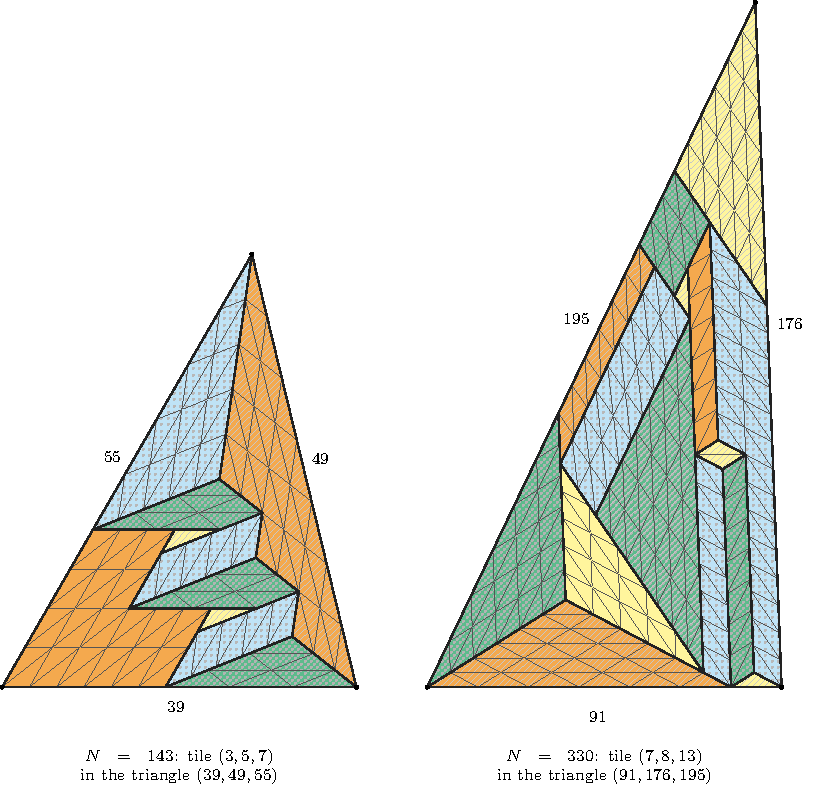
\includegraphics[trim=0 0 200bp 130bp,clip,width=0.5\linewidth]{figures/fig_143.pdf}
\caption{The tiling of the triangle $(39,49,55)$ by $143$ copies of $(3,5,7)$ (angle $2\pi/3$ between the sides $3$ and $5$), the sporadic count $143$ of $F_4$; it was found by a search in an earlier release and is a Lean theorem there. $143$ is not of any of the forms $k^2$, $x^2+y^2$, $3k^2$, $6k^2$ and is in no parametric family of this paper. Colours are orientation classes (same colour: tiles related by translation or half-turn); hatched: mirror images.}\label{fig:t143}
\end{figure}

\subsection{What is proved about C}
\begin{theorem}[The existence half, on the proved ranges; \PL{}]\label{thm:Cexist}
Let $\mathrm{ConjCBase}(N)$ be the statement ``$N=k^2n$, $k\ge1$, $n$ in the Lean predicate $F_0\cup\dots\cup F_6$ with the ranges proved at the time of that module''. Then $\mathrm{ConjCBase}(N)$ implies that $N$ is a tile count.
\end{theorem}
\emph{Lean:} \lean{ConjC.Exist.conjC_existence} (modules \texttt{ConjC/Defs}, \texttt{ConjC/Exist}, \texttt{ConjC/BetaCount}; aggregate \lean{AllConjC}; each family predicate is exactly the parameter range of an existing Lean existence theorem, and the non-vacuity of each is checked on an instance, e.g.\ \lean{conjCBase_143}, \lean{conjCBase_11625}). It collects constructions under one statement; it is not new mathematics beyond the family theorems it cites.
The predicate in Lean is narrower than Table~\ref{tab:families}: it has $F_1$ for $M\ge f$ only (Theorem~\ref{thm:W}, the tails and the macro counts of Sections~\ref{sec:collar}--\ref{sec:macro} are separate Lean theorems, not yet folded into it), it has no $F_7$, $F_8$, and its $F_5$ is the part proved at the time (the row $e=1$, $g\ge f+1$; $966g^2$, $g\ge25$; five engine values; the better tail $g\ge17$ of Theorem~\ref{thm:tails}(c) is a separate theorem not folded into this predicate).

\medskip
\noindent\CE{} \emph{Consistency checks} (exact computations in the working notes, repeated for the census of this release where stated).
(a) The families generate exactly the $105$ tile counts $\le200$ of the earlier theorem, no more and no fewer.
(b) None of the $199\,364$ Lean-formal excluded values of the census is generated by any family (rechecked for the Theorem~W family and the macro counts in this release: no overlap).
(c) Every one of the known tile counts of the census is generated by some family; this check is partly circular, because the known values were found by these families, so it shows that the families are complete for what is known and nothing more.
The sharp content of C is the exclusion half.

\subsection{What the exclusion half needs}
Everything proved in the exclusion direction in the earlier releases is compatible with C. The exclusion half of C is not proved: it is the statement that no value outside the families is a tile count, and it decomposes into threshold statements, one for each family at the place where the known range stops:
\begin{itemize}
\item[$W^*$] for $F_1$ with $2\le e\le f-2$: $W_M(e,f)$ is tiled iff $M\ge M^*(e,f)$; open for $e>f/2$ (Section~\ref{sec:thmW}); and $T^*$: $T_M$ is tiled iff $W_M$ is.
\item[$V,A'$] for $F_6$: the target $\Omega_g$ of $\gamma=2\alpha$ is tiled only if $v\mid g$, and for $g=1$, $(g-1)(v-u)<u$; open.
\item[$\Theta$] for $F_8$: $\theta_t(e,f)$ is tiled iff $t$ is in a semigroup, with $te<2f$ excluded (proved, \PL{}).
\item[$S_3$] for $F_5$: the row $G(e,f)$ has a smallest element $g_{\min}(e,f)$ and its gaps; known values are $g_{\min}(1,2)=2$ (exactly, since $21$ is not a tile count: every $N\le200$ is decided in the earlier release), $g_{\min}(2,5),\,g_{\min}(1,6)\in\{1,2\}$, $g_{\min}(1,4)\le5$.
\item[$Z$] for $F_3$: Zhang's counts $m^2a b$ etc.\ below the threshold $m<3t_0$ of the earlier release are not tile counts unless another family covers them; the known exceptions are the $15m^2$ and $33m^2$ counts.
\item small leaves: the $\pi/3$ and $2\pi/3$ pairs with irrational angle (closed, \PL{}), the commensurable cases.
\end{itemize}
Each of these is an infinite non-existence theorem; the methods of this project (additive invariants and the run induction of the earlier papers) prove them only in the ranges stated, and a count at a single scale cannot decide a threshold statement at all, because the same tile tiles the target at every larger scale.
\textbf{Expectation.} We expect the true set to be a union of schemas of this type, since a threshold or a semigroup appears in all constructions known; whether the thresholds $g_{\min}(e,f)$ and $M^*(e,f)$ have closed forms for all rows is open (for $F_1$, $W$ now has one).
If a core outside all families is ever found, C needs a further family and the classification becomes an open-ended census.
\textbf{Falsifiability.} The cheapest tests of C: the smallest value of $F_5$ outside the known range ($1860=465\cdot2^2$, $4185$, $7440$), the squarefree cores $465$, $966$, $2485$ ($g=1$; C predicts that they are not tile counts), and the first open value of $F_6$ at $g=v$, namely $1617=(4,7,g=7)$.

%=====================================================================
\section{The census}\label{sec:census}

\subsection{What it counts}
The universe is the $392\,074$ non-squarefree integers $N\in[2,10^6]$; $N$ is \emph{excluded} if the decidable arithmetic hypothesis of the single Lean theorem of the earlier paper (the exclusion theorem; it is not restated here) fails for it (a program evaluates the hypothesis for each $N$; the theorem is Lean, the evaluation is computation), \emph{known} if some construction gives a tiling, and \emph{undecided} otherwise.
The three sets are disjoint (asserted by the script: no known value is excluded).
The baseline is the census of the previous release.
\begin{center}\small
\begin{tabular}{@{}lrrr@{}}
\toprule
 & excluded & known (tile counts) & undecided\\
\midrule
version 2.2 / release v1.16 & $199\,140$ & $102\,613$ & $90\,321$\\
version 3.0 / release v3.0 (Lean-formal exclusions) & $199\,364$ & $129\,108$ & $63\,602$\\
change & $+224$ & $+26\,495$ & $-26\,719$\\
version 3.0 with the hand-proved class R2 (separate row) & $199\,441$ & $129\,108$ & $63\,525$\\
\bottomrule
\end{tabular}
\end{center}
The exclusion side grew by $224$ values: $124$ by the thick-regime theorem of Section~\ref{sec:thick}, $91$ by two further classes ($85$ values of the form $30s^2$ through the earlier gap lemma and $6$ values $t^2(12t^2-1)$ with $e=1$, $2M=f$), and $9$ from the re-run of the census program; the exclusion assignment is made by the census program, and only $412$ and $270$ below $1000$ are also Lean theorems about \emph{that} $N$ (\texttt{no\_dissection\_412}, \texttt{no\_dissection\_270}); the others are census-level (their leaf checks are too heavy for the kernel in the current interface). The row with Theorem~R2 adds $77$ values and is \emph{hand-proved}; do not read it as formal. The $26\,495$ new known values, by label:
\begin{center}\small
\begin{tabular}{@{}p{4.6cm}rp{6.0cm}@{}}
\toprule
label & values & source\\
\midrule
\PL{} (formal) & $26\,312$ & Theorem~\ref{thm:W} family ($26\,138$ new), collar and tails, macro counts, 13 W-below closures, $k^2$-multiples\\
\CE{} only (exact tiling, no Lean) & $145$ & witness-only values from template searches\\
\PH{} (hand) & $35$ & collar step with $h>1$ on the rows $(1,f),(2,3),(2,5)$ (Theorem~\ref{thm:collar})\\
paper-formal closure over exact seeds & $3$ & upward closure statement of the earlier paper over verified seeds\\
\bottomrule
\end{tabular}
\end{center}
(The $102\,613$ known values of the baseline keep the labels of the previous release.)
Theorem~W alone moves $26\,138$ values from undecided to known: the family has $44\,495$ values $\le10^6$ ($28\,946$ from $W$, $18\,431$ from $T$, union $44\,495$; the largest $f$ is $251$); $18\,357$ of them were already known by other means, none lies in the excluded set.
\textbf{Paliy-claim-only values.} A further $134$ values $\le10^6$ lie in families that Paliy claims (\CP{}; examples are $1380$, $2024$, $3105$, $4554$, $5520$, $8096$, and the values $15m^2$, $m\ge4$, that no Lean theorem covers, such as $1815=15\cdot11^2$) and that we have neither proved nor verified; they are \emph{not} counted as known, they are among the $63\,602$ undecided. The three values $1860$, $4185$, $7440$ ($465g^2$, $g=2,3,4$) were found after this census was run; they are exact-verified tile counts and are not in the table.

\subsection{Squarefree values}
Of the squarefree $N\le10^6$, about $770$ remain open at the exact level ($771$ in version~2.2: the difference is $4830$, a tile count by Paliy's certificate, exact-verified here); at the Lean level the count of the previous release ($791$) is unchanged, since all new Lean theorems concern non-squarefree values.
The open squarefree values $\le1000$ are $231,\ 329,\ 354,\ 385,\ 455,\ 465,\ 517,\ 777,\ 806,\ 935,\ 966$.
The undecided non-squarefree values in $[201,1000]$ were $38$ in the census of the first draft of this release; of these, $270$ and $412$ are now excluded by Lean theorems and $750$ and $963$ by the census program only, leaving $34$: $236$, $270$, $280$, $284$, $297$, $332$, $351$, $412$, $420$, $423$, $444$, $480$, $524$, $531$, $552$, $594$, $616$, $644$, $668$, $716$, $732$, $747$, $750$, $816$, $824$, $840$, $855$, $876$, $880$, $908$, $912$, $924$, $927$, $944$, $945$, $956$, $963$, $999$ ($414$ and $639$, tile counts of $W_3(2,5)$ and $T_3(2,5)$, are no longer on the list).
Every $N\le200$ was already decided.

\subsection{What the census is not}
It is not a classification: the undecided values may be tile counts or not. It rests on the families known to us; a tile count in a family we do not know is invisible to it.
The excluded values are excluded by Lean theorems, but the assignment ``this $N$ satisfies the hypothesis'' is made by a program, not by the kernel (as in the earlier paper).
The known values are of the stated labels; only the \PL{} ones are Lean theorems about \emph{that} $N$.

%=====================================================================
\section{Computer evidence on one open family: the $W^{3+}$ census}\label{app:w3}
This section records exact computations that are \emph{not} proofs and \emph{not} formal.
\subsection{The family and the question}
Let $u<v<2u$ be coprime, $b=v^2-u^2$, tile $(u^2,b,uv)$ (this is the family $F_6$, with $\gamma=2\alpha$), and $\Omega_g$ the isosceles target with base angles $\alpha$, legs $gub$, base $gvb$; a tiling has $g^2b$ tiles.
The earlier papers prove that $\Omega_g$ is not tiled when $(g-1)(v-u)<u$ (Theorem~F) and conjecture that it is tiled only if $v\mid g$ ($V$) and $g\ge g_D(u,v)$ ($A'$); the only tilings known are three Herdt-type counts, $1125$, $19\,600$, $130\,977$.
Two open instances with $v\nmid g$ and $(g-1)(v-u)\ge u$ are $g=3$ for $(u,v)=(4,7)$ (tile $(16,33,28)$, $N=297$) and $(5,8)$ (tile $(25,39,40)$, $N=351$).

\subsection{The words}
In a tiling of $\Omega_g$, the tiles with an edge on a leg partition the leg into segments; reading from the corner $\alpha$ to the apex gives a \emph{word}: the sequence of edge letters ($a$, $b$ or $c$) with the angles of the tiles at their ends.
The length of the leg and the angle sums at the ends leave a finite list of admissible words; hand-proved filters (named in the working notes; they are not the conjecture $A'$ above) and a rule for the junction at the apex cut it down to the set we call \emph{$W^{3+}$}.
For each word an exhaustive exact search (integer arithmetic, no floating point) asks whether the part of a tiling near that leg exists.
The verdict ``no tiling'' for a word is therefore conditional on the filters; it covers every tiling whose leg word is that word, and \emph{only} such tilings (it is not a verdict on $\Omega_g$ unless it is returned for every word, including the words outside $W^{3+}$ that the filters exclude).
\begin{center}\small
\begin{tabular}{@{}lrrrr@{}}
\toprule
$(u,v)$, $g=3$ & words & no tiling & tiling found & open\\
\midrule
$(4,7)$ & $191\,940$ (complete list) & $191\,940$ & $0$ & $0$\\
$(5,8)$ & $84\,462$ (complete list) & $84\,462$ & $0$ & $0$\\
$(7,12)$ & $8\,431\,936\,799$ & $8\,014\,982\,151$ ($95.06\%$) & $0$ & $416\,954\,648$\\
\bottomrule
\end{tabular}
\end{center}
For $(4,7)$ and $(5,8)$: all but $323$ and $630$ words fall within $2$ s each; the remainder were rerun at $120$ s, $1800$ s, and without a time limit (the two hardest words of $(4,7)$ took $5614$ s and $3269$ s); every word is decided.
For $(7,12)$ the word list has $8.4\times10^9$ entries and was covered by an adaptive prefix tree (a ``no tiling'' for a prefix refutes all its completions: the justification is that no tile edge straddles the end of a word prefix); the residual $4.2\times10^8$ words are open and the run was stopped because the fraction of prefixes that time out grew with depth.
\textbf{Controls.} The search finds the known tilings when it is given their own words (the words of the tilings of the scaled tile at $m=3,4$, for all three pairs: found and verified), and refutes the reversed words and words refuted independently by a slower program.
\textbf{What this shows and does not show.} No tiling was found, so $V$ and $A'$ are not refuted. It does not show that $297$ and $351$ are not tile counts, because the verdict is for the one-leg word set, not for all tilings and all shapes of target; and without a Lean certificate it is not a theorem. It is evidence, and it narrows where a counterexample could be.


%=====================================================================
\section{Corrections of earlier statements}\label{app:corr}
Statements made in our working notes, and in one case in an earlier release, that this paper corrects. None of the corrections affects a Lean theorem, a prime-case statement or an excluded value of the census.
\begin{enumerate}
\item \textbf{$183$ is not a tile count.} An earlier draft of the conjecture listed $183$ as a sporadic tile count (attributed to Laczkovich). $183$ is excluded, and every $N\le200$ is decided in Lean; the draft misread a statement about $5\cdot183^2$. The Lean predicate $F_4$ never contained it.
\item \textbf{Tiles of $T_M$ and $W_M$ below the scale $f$ exist for $e\ge2$.} Our notes asserted that $T_M(e,f)$ and $W_M(e,f)$ have no tiling for $M<f$ when $e\ge2$ (``$B_1$''), and that the $T$ half of this statement stood after the $W$ half failed. Both are false: Theorem~\ref{thm:W} and the glue of Paper~W, Section 3.3. The version 1 paper \cite{ReleasePaper} recorded, as an observation, that ``in every case decided so far'' the scale $f$ is the threshold; Corollary~\ref{cor:W435} is a counterexample ($W_4(3,5)$, $M=4<5$). The open problems of that paper on the scales $f/(2e)<M<f$ are partly closed here (Section~\ref{sec:thmW}).
\item \textbf{The template ``exists iff $4f<9e$'' is false.} An intermediate note (13 witnesses below $f$, then a replay of one search) stated that the six-piece template exists only for $4f<9e$, was absent for $432$ coprime pairs with $f\le60$, and that the conjectured threshold held only there. This was an artefact: the replay of one search history has an empty cone for the other pairs, but the geometry of the same six pieces works for all $2\le e\le f-2$ (Theorem~\ref{thm:W}; for $(2,5)$, $(3,7)$, $(4,9)$, $(5,12)$, $(3,8)$ the tilings exist).
\item \textbf{The size conjecture is false.} The working notes (and a conjecture in a longer draft) stated that a target not similar to the tile has longest side at least $c^2=f^4$. $W_4(3,5)$ has longest side $500<625$.
\item \textbf{Paliy's $4830$ is a tiling.} Our notes said that his $4830$-tile file is not a tiling. We had checked the wrong file (his refuted moment counterexample, not his certificate). His certificate, $4830$ copies of $(24,11,31)$ on the triangle $(961,1155,1426)$, is verified exactly (Section~\ref{sec:macro}).
\item \textbf{The $\theta$-isosceles statement.} Our notes stated ``targets $\theta_t(e,f)$ with $te\ge f$ have no tiling''. That is false: $\theta_4(1,2)$ and $\theta_8(2,3)$ are tiled. The proved statement is the necessary bound $te\ge2f$; the true statement is a threshold (a semigroup of scales, Paliy), not an exclusion.
\item \textbf{Priority of the $\alpha$ up-set.} The up-set in $g$ of the base-$\alpha$ rows and the form $b\kappa K^2$ are Paliy's, dated 29 September 2026 (Section~\ref{sec:collar}); our notes had presented the up-set as ours. The scale additivity of the rows is also his.
\item \textbf{The collar corollary has two conditions.} The first version of the statement ``$g_0$ in the row implies every $g\ge g_0$ is in the row'' in our notes used only $h_{\max}(g_0)\ge g_0-1$; the audit added $h_{\max}(x)\ge1$ for $x\ge2g_0-1$.
\item \textbf{Counts in a note.} The census effect of the collar step was first stated as $235$ values; the correct figure, by an audit that recounted, was $194$ ($119$ in the rows $(1,f),(2,5)$ and $75$ in $(2,3)$); the figures of this release supersede both.
\item \textbf{The threshold formula $(M-1)(f-e)\ge f$.} Used as a threshold for all rows it contradicts the proved side theorem $W_M$ none if $Me<f$ exactly when $\lceil f/e\rceil>\lceil f/(f-e)\rceil+1$ (for instance $(2,7)$: the formula gives $M=3$, but $3\cdot2<7$). The correct threshold is $M^*(e,f)=\max(\lceil f/e\rceil,\lceil f/(f-e)\rceil+1)$.
\item \textbf{The pattern $g_{\min}=f+1$.} Our notes observed that the first realised scale of a base-$\alpha$ row was $f+1$ for even $f$ and recorded this as a pattern; $g_{\min}(1,6)\le2$ (Theorem~\ref{thm:tails}) refutes it ($f=6$ is even), and $g_{\min}(2,5)\le2$ as well.
\end{enumerate}
The register of corrections of the project is in the repository (file \texttt{TIMELINE.md} records the dates).

%=====================================================================
\section{Data: the explicit tilings}\label{app:data}
\subsection{The thirteen first witnesses with $M<f$}
Found first by a computer search, and now instances of Theorem~\ref{thm:W}; every one is a Lean theorem (module \texttt{Draft/DebtBWTilable}, with the closure upward in $M$).
\begin{center}\small
\begin{tabular}{@{}lrr@{\qquad}lrr@{}}
\toprule
$(e,f,M)$ & $W_M$ tiles & $T_M$ tiles & $(e,f,M)$ & $W_M$ tiles & $T_M$ tiles\\
\midrule
$(3,5,4)$ & $656$ & $1056$ & $(7,12,4)$ & $3824$ & $6128$\\
$(4,7,4)$ & $1312$ & $2096$ & $(7,10,5)$ & $3775$ & $6275$\\
$(5,8,4)$ & $1648$ & $2672$ & $(7,9,6)$ & $4068$ & $6984$\\
$(5,7,5)$ & $1825$ & $3050$ & $(8,11,5)$ & $4450$ & $7475$\\
$(5,11,3)$ & $1953$ & $3042$ & $(9,11,7)$ & $7889$ & $13\,818$\\
$(5,9,4)$ & $2192$ & $3488$ & $(6,11,4)$ & $3296$ & $5232$\\
$(7,11,4)$ & $3088$ & $5024$ & & &\\
\bottomrule
\end{tabular}
\end{center}
\subsection{The shipped files}
Directory \lean{data/witnesses/v3_exact}: $97$ files, each named by the number of tiles, the kind and the parameters (for example \lean{tiling_414_W_2_5_M3.exact.txt.gz}). Each begins with a comment line stating the number of tiles and the side lengths of the tile; every other line gives the three vertices of one tile in exact rational coordinates $(X,Y\sqrt D)$. Kinds: \texttt{W}, \texttt{T} (Theorem~W and its glue: $37$ and $15$ files), \texttt{collar} ($6$) and \texttt{macro} ($38$) (Sections~\ref{sec:collar}, \ref{sec:macro}), \texttt{F3\_paliy} (Paliy's $4830$). Verification: the exact verifier of the repository (\texttt{bte verify}) reports, for each file, that the tiles are congruent to the stated tile, that their interiors are pairwise disjoint, that the total area equals the area of the hull, and that the hull is a triangle. All $97$ pass.

\section{Index of the Lean statements}\label{app:lean}
All in the library of the repository (directory \texttt{lean/}); aggregate \lean{Erdos634.AllV3} (the modules new in this release; build one module at a time through \texttt{code/lakeserial.py}); the axioms of $98$ of them are printed by \texttt{lean/axioms/AxiomsAllV3.lean} and every line reads \texttt{[propext, Classical.choice, Quot.sound]}.
\begin{center}\small
\begin{tabular}{@{}p{4.9cm}p{8.1cm}@{}}
\toprule
statement & Lean name (namespace \texttt{Erdos634.}\dots)\\
\midrule
Theorem~\ref{thm:W} & \lean{Draft.ThmW.thmW}; counts \lean{Draft.ThmW.tileCount_W}, \lean{tileCount_T}; examples \lean{inst_414}, \lean{inst_656}, \lean{inst_639}, \lean{inst_27324}\\
13 first witnesses, closures & \lean{Draft.DebtB.closure_656} etc.; \lean{DebtB.counts_of_wTilable}\\
Collar layer step & \lean{Draft.CollarLayer.layer_core}, \lean{Draft.CollarFam.layer_step}\\
Theorem~\ref{thm:seedA} & \lean{Draft.CollarUp.tileCount_e1_up}; instances \lean{tileCount_189}, \lean{tileCount_16740}, \lean{tileCount_159040}\\
Theorem~\ref{thm:tails} & \lean{Draft.CollarFam.tileCount_465_sq}, \lean{Draft.CollarFam5.tileCount_2485_sq5}, \lean{Draft.CollarFam17.tileCount_966_sq17}\\
Macro pieces (Thm~\ref{thm:macro}) & \lean{Draft.MacroPiece.macroTFam_gen}; \lean{Draft.TM375.tileCount_375} etc.; \lean{Draft.T62125.tileCount_62125}; \lean{Draft.AllMacro.tileCount_78246}\\
Twelve square multiples & \lean{Draft.TemplateSquares.tileCount_46500} etc.\\
Conjecture C, existence half & \lean{ConjC.Exist.conjC_existence}; \lean{ConjC.BetaCount.tileCount_beta_ge}\\
\bottomrule
\end{tabular}
\end{center}

\section{Reproducing the checks}\label{app:repro}
From a clean clone, with the toolchain of \texttt{lean/lean-toolchain}: build the aggregate one module at a time, print the axioms, and verify the exact tilings:
\begin{verbatim}
python3 code/lakeserial.py lean build Erdos634.AllV3
(cd lean && lake env lean axioms/AxiomsAllV3.lean) \
   | python3 code/axiom_gate.py
BTE=rust/bonfioli_tiling_engine/target/release/bte
for f in data/witnesses/v3_exact/*.gz; do
  $BTE verify "$f" | grep -q VERIFIED || echo FAIL "$f"
done
\end{verbatim}
The build needs about $6$ GB of memory for its largest module and about $22$ GB of disk for the build products; one module is built at a time. The scripts \texttt{code/reproduce.sh} (all earlier checks) and the above give the complete set.

%=====================================================================
\begin{thebibliography}{99}
\bibitem{BeesonI} M.~Beeson, \emph{Triangle tiling I: The tile is similar to ABC or has a right angle}, arXiv:1206.2231.
\bibitem{BeesonRosu} M.~Beeson and G.~Ro\c{s}u, \emph{Tiling a triangle into a prime number of congruent triangles}, preprint, version of 16 October 2026.
\bibitem{BeesonIII} M.~Beeson, \emph{Triangle tiling III: the case $3\alpha+2\beta=\pi$}, arXiv:1206.2229.
\bibitem{BeesonIso} M.~Beeson, \emph{Tilings of an isosceles triangle}, arXiv:1206.1974.
\bibitem{BeesonWithdrawn} M.~Beeson, \emph{No prime tiling of an isosceles triangle}, arXiv:2607.19572 (withdrawn in version 2, 24 September 2026, with a note attributing the theorem to V.~Bonfioli).
\bibitem{Erdos633} M.~Beeson, M.~Laczkovich and Y.~X.~Zhang, \emph{Solution of Erd\H{o}s Problem~633}, arXiv:2604.03609.
\bibitem{Laczkovich1995} M.~Laczkovich, \emph{Tilings of triangles}, Discrete Math.\ \textbf{140} (1995), 79--94.
\bibitem{Laczkovich2012} M.~Laczkovich, \emph{Tilings of convex polygons with congruent triangles}, Discrete Comput.\ Geom.\ \textbf{48} (2012), 330--372.
\bibitem{PaliyPrime} D.~Paliy, \emph{No scale-one triangle in either rational Group-1 family}, and the deduction of the prime case, repository \texttt{github.com/DenisUkranian/erdos-634-tilings}, files \texttt{docs/prime-case-candidate.md} and \texttt{docs/prime-case-dependencies.md}, first published 29 September 2026; unrefereed.
\bibitem{PaliyRepo} D.~Paliy, repository \texttt{github.com/DenisUkranian/erdos-634-tilings}: notes on eventual rational families (\texttt{docs/eventual-rational-families.md}), the $\theta$-branch (\texttt{docs/theta-branch.md}), the $W/\beta$ framework and the macro-dissection files, September--October 2026; unrefereed.
\bibitem{PaperW} V.~Bonfioli, \emph{Tilings of $W_M$ and $T_M$ below the threshold scale: a six-piece template} (Paper~W), version 3.0, release v3.0.
\bibitem{ReleasePaper} V.~Bonfioli, \emph{Congruent dissections of a triangle: prime counts, the counts up to $200$, and a family of isosceles targets}, release v1.13.1, Zenodo, October 2026 (concept DOI of all versions: doi:10.5281/zenodo.23400433).
\bibitem{Release22} V.~Bonfioli, \emph{Congruent dissections of a triangle: runs, windows and the corner}, version 2.2, release v1.16, Zenodo (same concept DOI, version tag v1.16).
\bibitem{SWW} S.~L.~Snover, C.~Waiveris and J.~K.~Williams, \emph{Rep-tiling for triangles}, Discrete Math.\ \textbf{91} (1991), 193--200.
\bibitem{Soifer} A.~Soifer, \emph{How does one cut a triangle?}, 2nd ed., Springer, 2009.
\bibitem{Zhang} Y.~X.~Zhang, \emph{Tiling triangles with $2\pi/3$ angles}, arXiv:2512.22696.
\end{thebibliography}

\end{document}
